\documentclass{beamer}
\usepackage{../common_slides}


\title{Text Classification\\ + \\ Machine Learning Review }

\author{Alexander Rush}
\begin{document}


\begin{frame}
  \titlepage
\end{frame}

\section{Text Classification }

\begin{frame}{Application: Spam Detection}

\end{frame}

\begin{frame}{Application: Topic Detection}

\end{frame}

\begin{frame}{Application: Sentiment Analysis}
  
\end{frame}

\begin{frame}{Why?}
  \begin{itemize}
  \item Easy problem.
  \end{itemize}
  \begin{itemize}
  \item Surface-level
  \end{itemize}
\end{frame}

\begin{frame}{Task: Text Classification}

  Given a sentence determine its class, 

  Bad Sentences

  Unfortunately the story and the actors are served with a hack script. 
  A sentimental mess that never rings true.
  This 100-minute movie only has about 25 minutes of decent material.  
  Here, common sense flies out the window, along with the hail of bullets, none of which ever seem to hit Sascha. 

  Good Sentences
  
  A thoughtful, provocative, insistently humanizing film. 
  Occasionally melodramatic, it's also extremely effective.
  Guaranteed to move anyone who ever shook, rattled, or rolled.   
\end{frame}


\section{Machine Learning Preliminaries}

\subsection{Features and Preprocessing}

\begin{frame}{Preliminary Notation}
  \begin{itemize}
  \item $\boldb, \boldm$;  bold letters for vectors.
  \item $\boldB, \boldM$;  bold capital letters for matrices.
  \item $\mcB, \mcM$;  script-case for sets.
  \item $B, M$; capital letters for constants and random variables.
  \item $b_i, x_i$; lower case for scalars or indexing into vectors.
  \end{itemize}


  \begin{itemize}
  \item $\bolddelta(i)$; one-hot vector at position i
    \[\bolddelta(2) = \left[ 0; 1; 0; \dots \right]\] 
  \item $\indicator(x = y)$; indicator 1 if $x = y$, o.w. 0

  \end{itemize}


\end{frame}


\begin{frame}{Text Classification}
  How do we do this? 

  \begin{enumerate}
  \item First extract information from the sentence. 
  \item Use this to construct a \textit{representation}
  \item Classify this vector is the set of possible outputs.
  \end{enumerate}

  % Throughout this class, 
  % \begin{itemize}
  % \item $\mcX = \reals^{\din}$
  % \item $\mcY \subset \{0, 1\}^{\dout}$
  % \end{itemize}
\end{frame}





\begin{frame}{Input Representation}
  \begin{itemize}
  \item How do we convert an input sentence into a usable mathematical representation?
  \item Main focus of this class, representation of language
  \item Point in coming lectures: \textit{sparse} vs. \textit{dense} representations
  \end{itemize}
\end{frame}


\begin{frame}{Sparse Features}
  \begin{itemize}
  \item   Define $\mcF$ to be a discrete set of predefined features. 
  \item   For a given sentence, let $f_1\in\mcF, \ldots , f_k\in\mcF$ be the relevant features. 
    Typically $k << |\mcF|$.
  \item Define the sparse representation of the input
    \[\boldx = \sum_{i=1}^k \bolddelta(f_i) \]
  \item $\boldx \in \reals^{1\times \din}$; input representation 
  \end{itemize}

  % In this section we consider \textbf{sparse} features. Informally this means
  % $\din$ is large, and $\boldx$ is sparse.   
\end{frame}



\begin{frame}{Features 1: Sparse Bag-of-Words Features}
  Representation is indicators of input words, 
  \begin{itemize}
  \item $\mcF$; the vocabulary of the language.
  \item $\boldx = \sum_{i} \bolddelta(f_i)$ 
  \end{itemize}

  Example: Movie Sentiment
  \begin{center}
    \texttt{A sentimental mess}
    \[ \boldx = v(\texttt{word:A}) + v(\texttt{word:sentimental}) +
    v(\texttt{word:mess}) \] 
    \[ \boldx^\top =\begin{bmatrix} 1 \\ \vdots
        \\ 0\\ 0 \\ \end{bmatrix} +\begin{bmatrix} 0 \\
        \vdots \\ 0\\ 1 \\ \end{bmatrix} +
     \begin{bmatrix} 0 \\ \vdots \\ 1\\ 0 \\ \end{bmatrix} 
    =\begin{bmatrix} 1 \\ \vdots \\ 1 \\ 1 \\ \end{bmatrix} 
    \begin{matrix*}[l] \mathrm{\texttt{word:A}} \\ \vdots \\ \mathrm{\texttt{word:mess}} \\ \mathrm{\texttt{word:sentimental}} \\ \end{matrix*}
     \]
  \end{center}
\end{frame}


\begin{frame}{Features 2: Sparse Word Properties}
  Representation can use specific aspects of text.
  \begin{itemize}
  \item $\mcF$; Spelling, inner-word capitals, trigger words, etc. 
  \item $\boldx = \sum_{i} \bolddelta(f_i)$ 
  \end{itemize}

  Example: Spam Classification

  \begin{center}
    \texttt{Your diploma puts a UUniversity Job Placement Counselor at
      your disposal.}
  \end{center}
  \[  \boldx = v(\texttt{misspelling}) + v(\texttt{capital}) + v(\texttt{word:diploma}) + \ldots\]
  \[
  \boldx^\top = 
 \begin{bmatrix} 0 \\ \vdots \\ 0\\  0 \\  \end{bmatrix} + 
 \begin{bmatrix} 0 \\ \vdots \\ 1\\ 0 \\  \end{bmatrix} +
 \begin{bmatrix} 0 \\ \vdots \\ 0\\  1 \\  \end{bmatrix} = 
 \begin{bmatrix} 1 \\ \vdots \\ 1 \\ 1 \\  \end{bmatrix}     \begin{matrix*}[l] \mathrm{\texttt{misspelling}} \\ \vdots \\ \mathrm{\texttt{capital}} \\ \mathrm{\texttt{word:diploma}} \\ \end{matrix*}
  \]
\end{frame}

\subsection{Output}

\begin{frame}{Output Representation}
  \begin{itemize}
  \item How do we handle the output representation?
  \item We will use a one-hot output encoding (may be slightly different).
  \item In future lectures, efficiency of output encoding.
  \end{itemize}
\end{frame}




\begin{frame}{Output Classes}
  \begin{itemize}
  \item $\mcC = \{1, \ldots, \dout\}$; possible output classes
  \item $c \in \mcC$; the true output class 
  \item $\boldy = \bolddelta(c) \in \reals^{1\times \din}$; one-hot output representation

  \item Note: when classes are words, we call them \textit{word types}. 
  \end{itemize}
\end{frame}

\begin{frame}{Output Form: Binary Classification}

  Examples: spam/not-spam, good review/bad review, relevant/irrelevant document, many others.   
  \begin{itemize}
  \item $\dout = 2$; two possible classes
  \item In our notation,
    \begin{eqnarray*} 
    c = 1 & \  \boldy &= \begin{bmatrix} 1 & 0  \end{bmatrix}  \mathrm {\ vs. \ } \\
    c = 2 & \boldy &= \begin{bmatrix} 0  & 1  \end{bmatrix} 
   \end{eqnarray*} 
   \item Can also use a single output \textit{sign} representation with $\dout = 1$ 
  \end{itemize}

\end{frame}


% \begin{frame}{Step 1: Feature Extraction}
%   \begin{itemize}
%   \item Let $\mcV$ be the vocabulary of our language.  
%   \item  Let $w_1, \ldots, w_m$ be a sentence, where 
%     $w_i \in \{1,\ldots, |\mcV|\}$.
%   \item 
%   \end{itemize}
% \end{frame}



% \begin{frame}{Step 2: Learn a Classifier}
%   Next we map a representation $\boldx$ to a output $\boldy$.
  
%   The output $\boldy \in \reals^\dout$ where $\dout$ is the number of 
%   \textit{classes}. 

%   Generally $\boldy$ will be a one-hot vector. 

%   \begin{itemize}
%   \item $\dout = 2$; two possible classes
%     \[\begin{bmatrix} 1 \\ 0  \end{bmatrix}  \mathrm {\ vs. \ } 
%    \begin{bmatrix} 0 \\ 1  \end{bmatrix} \]
%   \end{itemize}

%   For instance spam/not-spam, good review/bad review, relevant/irrelevant

% \end{frame}

\begin{frame}{Output Form: Multiclass Classification}
  Examples: Yelp stars, etc.
  \begin{itemize}
  \item $\dout = 5$; for examples
  \item In our notation, one star, two star...
    \begin{eqnarray*} 
    c = 1 & \  \boldy &= \begin{bmatrix} 1 & 0 & 0 & 0 & 0  \end{bmatrix}  \mathrm {\ vs. \ } \\
    c = 2 & \boldy &=    \begin{bmatrix} 0 & 1 & 0 & 0 & 0 \end{bmatrix} \ldots
   \end{eqnarray*} 
  \end{itemize}
  Examples: Word Prediction (Unit 3)
  \begin{itemize}
  \item $\dout > 100,000$; 
  \item In our notation, $\mcC$ is vocabulary and each $c$ is a word.   
    \begin{eqnarray*} 
    c = 1 & \  \boldy &= \begin{bmatrix} 1 & 0 & 0 & 0 & \ldots & 0  \end{bmatrix}  \mathrm {\ vs. \ } \\
    c = 2 & \boldy &=    \begin{bmatrix} 0 & 1 & 0 & 0 & \ldots & 0 \end{bmatrix} \ldots
   \end{eqnarray*} 
  \end{itemize}
\end{frame}

\begin{frame}{Evaluation}
  \begin{itemize}
  \item Consider evaluating accuracy on outputs $\boldy_1, \ldots, \boldy_n$. 

  \item Given a decisions $\hat{c_1} \ldots \hat{c_n}$ we measure 
  accuracy as,
  
  \[ \sum_{i=1}^n \frac{\indicator(\bolddelta(\hat{c}_i) = \boldy_i)}{ n} \] 

  \item Simplest of  several different metrics we will explore in the class. 
  \end{itemize}
\end{frame}


% \begin{frame}{Example: Multiclass Classification}
%   More interestingly we will also consider multiclass where $\dout > 2$

%   \begin{itemize}
%   \item $\dout = 5$; yelp review.
%     \[\begin{bmatrix} 1 \\ 0 \\0 \\0 \\0  \end{bmatrix}  \mathrm {\ vs. \ } 
%    \begin{bmatrix} 0 \\ 1 \\0 \\0 \\0  \end{bmatrix}  \mathrm {\ vs. \ } \ldots \] 
%   \end{itemize}
%   For instance five star review, etc. 
% \end{frame}




\section{Classification}


\begin{frame}{Supervised Machine Learning}
  Let, 
  \begin{itemize}
  \item $(\boldx_1, \boldy_1), \ldots, (\boldx_n, \boldy_n)$; supervised data
  \item $\boldx_i \in \reals^{1 \times \din}$;  input representations  
  \item $\boldy_i \in \reals^{1 \times \dout}$; gold output representations (one-hot vectors)
  \end{itemize}

  Goal: Learn a classifier from input to output classes $\mcC$.  

  \air
  \air

  (Practically, store design matrix $\boldX \in \reals^{n
    \times \din}$ and output classes.)
\end{frame}


\begin{frame}{Review: Experimental Setup}
  
  \begin{itemize}
  \item Data is split into three parts training, validation, and test.
  \item Experiments are all run on training and validation, test is final output.

  \item (For assignments we will distribute training and validation, and only give $\boldx$ for test.)
  \end{itemize}
  
  For small text classification data sets,
  \begin{itemize}
  \item Even more careful. Results are reported with K-fold cross-validation. 
    \begin{enumerate}
    \item Split into K folds (equal splits).
    \item For each fold, train on other K-1 folds, test on current fold. 
    \end{enumerate}
  \end{itemize}
\end{frame}


\begin{frame}{Linear Models for Classification}
  Define a linear model as,
  \begin{itemize}
  \item Model, \[\hat{\boldy} = \boldx \boldW + \boldb\]   
  \item $\boldW \in \reals^{\din \times \dout}, \boldb \in \reals^{1 \times \dout}$; model parameters
  \item Note $\hat{\boldy}$ is \textbf{not} one-hot, informally ``score'' vector. 
  \end{itemize}

  The decision rule is then,
  \[ \hat{c} = \argmax_{i \in \mcC} \hat{y_i} \]
\end{frame}


\begin{frame}{Interpreting Linear Models}
  Parameters give scores to possible outputs,
  \begin{itemize}
  \item $W_{f, i}$ is the score for feature $f$ under class $i$
  \item $b_c$ is a prior score for class $i$  
  \item $y_i$ is the total score for class $i$
  \item $\hat{c}$ is highest scoring class under the linear model.
  \end{itemize}

  Examples:
  \begin{itemize}
  \item For feature score, \[[\beta_1, \beta_2 ] = \bolddelta(\texttt{word:dreadful}) \boldW,\]
    You would expect $\beta_2 > \beta_1$ (assuming $c=2$ is ``positive''). 
    
  \end{itemize}
\end{frame}

\subsection{Probabilistic Linear Models}

\begin{frame}{Probabilistic Linear Models} 
  % Estimate
  We can begin by interpreting prediction probabilistically,

  \begin{itemize}
  \item Let output be a random variable $Y$, with sample space $\mcC$. 
  \item Representation be a random vector $X$. 
  \item Interested in estimating parameters $\theta$ of, 
    \[ P(Y | X; \theta) \] 
  \end{itemize}
  We will be informal and use $p(\boldy=c | \boldx)$ for 
  $P(Y = c | X = \boldx)$.
  
\end{frame}



\begin{frame}{Probabilistic Linear Models} 
  % Estimate 
  \begin{itemize}
  \item $(\boldx_1, \boldy_1), \ldots, (\boldx_n, \boldy_n)$; supervised data
  \item Select parameters to maximize likelihood of training data.
    \[ \mathcal{L}(\theta) = - \sum_{i=1}^n \log p(\boldy_i | \boldx_i; \theta) \] 
  For linear models $\theta = (\boldW, \boldb)$ 

  \item Do this by minimizing negative log-likelihood.
    \[ \argmin_\theta \mathcal{L}(\theta)\] 
  \end{itemize}

\end{frame}

\begin{frame}{Properties: Probabilistic Model}
  \begin{itemize}
  \item Gives more than 
  \item Allows variant decision rules (for instance minimum bayes' risk)
  \end{itemize}
  
  \begin{itemize}
  \item May be less efficient to train. 
  \item 
  \end{itemize}
\end{frame}



\subsection{Linear Model 1: Naive Bayes}

\begin{frame}{Probabilistic Factorization} 
  % Estimate 
  Reminder, Bayes Rule

  \[ p(\boldy | \boldx) = \frac{p(\boldx | \boldy) p(\boldy)}{p(\boldx)} \] 

  Can be instead written (with $\propto$ as normalizing factor) 

  \[ p(\boldy | \boldx) \propto p(\boldx | \boldy) p(\boldy) \] 

  % Read as \textbf{posterior} is proportional to \textbf{likelihood} times 
  % the \textbf{prior}.

  For NLL, $p(\boldx)$ doesn't matter, estimate likelihood $p(\boldx | \boldy)$ and
  prior $p(\boldy)$.


  \air

  For a sparse model, we write, 
  
  \[p(x_{f_1}=1, \ldots, x_{f_k}=1 | \boldy=c ) p(\boldy=c)\]



\end{frame}


\begin{frame}{Naive Bayes Assumption} 

  \begin{eqnarray*}
    && p(x_{f_1}=1, \ldots, x_{f_k}=1 | \boldy=c ) p(\boldy=c) =\\
     && \prod_{i=1}^k p(x_{f_i}=1 | x_{f_1}=1, \ldots, x_{f_{i-1}}=1, \boldy=c) p(\boldy=c) \approx \\
     && \prod_{i=1}^k p(x_{f_i} | \boldy) p(\boldy)  
  \end{eqnarray*}

  
  First is by chain-rule, second is by assumption (Naive bayes). 

\end{frame}



\begin{frame}{Multinomial Model} 
  Brief aside, 
  \begin{itemize}
  \item $P(S; \theta)$; parameterized as a multinomial distribution (multinoulli in )  

  \item Minimizing NLL for multinomial for data has a closed-form.

    \[ \theta_s = \sum_{i=1}^n \frac{\indicator(s_i = s)}{n} \]

    \[ P(S=s; \theta) = \theta_s \]

  \item Exercise: Derive this by minimizing $\mathcal{L}$. 

  \end{itemize}
\end{frame}



\begin{frame}{Multinomial Naive Bayes}
  \begin{itemize}
  \item  Both the prior $p(\boldy = c)$ and the likelihood $p(\boldx | \boldy)$ are
    parameterized as multinomial (multinoulli) distributions.
    
  \item Fit prior as,
    \[p(\boldy = c) = \sum_{i = 1}^n \frac{1(\boldy_i = c)}{n}\]
    
  \item Fit likelihood as,
    \begin{itemize}
      \item Let \[F_{f,c} = \sum_{i = 1}^n \indicator(\boldy_i = c) \indicator(x_{i, f} = 1) \mathrm{\ for all\ } c\in \mcC, f\in \mcF\] 
      \item Then,
      
      \[p(x_f | \boldy=c) = \frac{F_{f, c}}{\displaystyle \sum_{f' \in \mcF} F_{f',c}}  \]     
    \end{itemize}
  \end{itemize}

    How does this become a linear classifier? 
  \[ W_{f, c} =  \log p(x_f = 1 | \boldy=c)  \] 
  \[ b_c = \log p(\boldy=c)  \mathrm{ for all  }c\in \mcY \] 

  So 
  \[\log p(\boldx | \boldy) p(\boldy) =  \boldx \boldW + \boldb  \]
\end{frame}


\begin{frame}{Digression: Zipf's Law}
  Word features ... 
\end{frame}

\begin{frame}{Laplacian Smoothing}
  \begin{itemize}
  \item   In order to handle the long tail of words. 
    Add a value of $\alpha$ to each element in the sample space before normalization.
    Where $\alpha$ is a smoothing hyperparameter 
  \item 
    \[ \theta_s =  \frac{\alpha + \sum_{i=1}^n \indicator{s_i = s}}{\alpha|\mcS| n} \]
    
  \item (Similar to Dirichlet prior in a Bayesian interpretation.) 
  \end{itemize}

  For naive Bayes:
  \begin{itemize}
  \item \[\hat{\boldF} = \alpha + F\]
  \end{itemize}
\end{frame}

\begin{frame}{Naive Bayes In Practice}
  
  % Results from paper.
  \begin{itemize}
  \item Incredibly fast
  \end{itemize}
\end{frame}

\subsection{Linear Model 2: Multiclass Logistic Regression}

\begin{frame}{The Softmax}

  Instead of factoring into multinomial, use a soft-max to force a distribution
  
  \[\softmax(\hat{\boldy}) = \frac{\exp(\hat{\boldy})}{\displaystyle \sum_{c \in \mcC} \exp(\hat{y})}  \]

  \begin{itemize}
  \item Exercise: Confirm always gives a distribution.

  \item Note denominator is known as the \textit{partition function}.
  \end{itemize}

\end{frame}


\begin{frame}{Why is it called softmax?}
  \[\softmax(\hat{\boldy}) = \frac{\exp(x)}{\displaystyle  \exp(x) + \exp(y)}  \]
  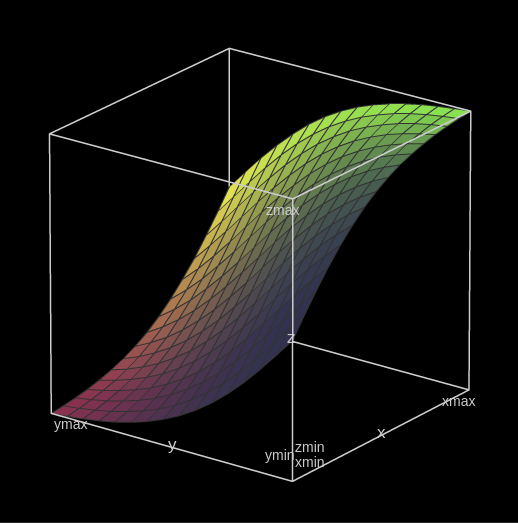
\includegraphics[width=5cm]{softmax}
  \[\argmax(\hat{\boldy}) = \indicator(x > y) \]
  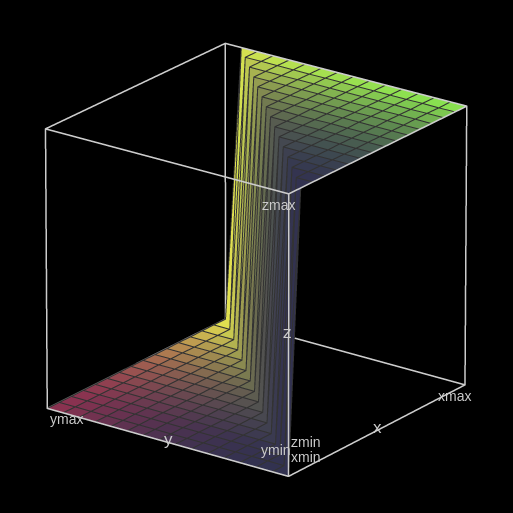
\includegraphics[width=5cm]{argmax}
\end{frame}

\begin{frame}{Multiclass logistic regression}
  
  \[ \hat{\boldy} = \boldx \boldW + \boldb\] 

    \[ p(\boldy =c | \boldx; \theta) = 
      \frac{\exp(\hat{\boldy_c})}{\displaystyle \sum_{\displaystyle c' \in \mcC} \exp(\hat{\boldy_{c'}})}   \] 
\end{frame}

\begin{frame}{Special Case: Binary Classification}
  For binary classification this is often 
  \begin{enumerate}
  \item   \[y = \boldx \boldW + b\]   
  \end{enumerate}

  \[ \softmax() = \frac{\exp(y_1)}{(\exp(y_1) + \exp(y_2))} = \frac{1}{1 + \exp{-(y_1-y_2)}} = \sigma(y_1 -y_2)\]

  
  Logistic sigmoid function

  \[\sigma(t) = \frac{1}{1 + \exp{-t}} \]
  
  Which is standard for logistic regression.
\end{frame}

\begin{frame}{A Model with Many Names}
  \begin{itemize}
  \item   Multinomial logistic regression

  \item Log-Linear (particularly in NLP)

  \item  Softmax Regression

  \item Max-Entropy ()
  \end{itemize}
\end{frame}


\begin{frame}{Benefits of Logistic Regression}
  \begin{itemize}
  \item 
  \end{itemize}
  \begin{itemize}
  \item Fitting parameters is much more difficult.
  \end{itemize}
  Models similar to LR will be the main focus of this class.
\end{frame}



\begin{frame}{Fitting Parameters}
  Recall probabilistic objective is:

  \[ \mathcal{L}(\theta) = - \sum_{i=1}^n \log p(\boldy_i | \boldx_i; \theta) \] 

  And the distribution is parameterized as a softmax,
  \begin{eqnarray*}
   \log p(\boldy=c | \boldx; \theta) &=& \log \softmax(\boldx \boldW  + \boldb)_c \\
    &=&\hat{y}_c - \log \sum_{c' \in \mcC} \exp(\hat{y}_{c'}) 
  \end{eqnarray*}

  However, this is much harder to solve, no closed-form.

  
\end{frame}


\begin{frame}{Computing Parameter Gradients}
  Consider one example $(\boldx, \boldy)$ maximizing $\log p(\boldy | \boldx; \theta)$, 

  \begin{enumerate}
  \item Compute scores $\hat{\boldy} =  \boldx \boldW + \boldb$  
  \item Compute log softmax of scores, $\log \softmax(\hat{\boldy})$  
  \item Compute gradient of $\mathcal{L}$ with respect to scores $\hat{\boldy}$ for all $c \in \mcC$ 

  \[\frac{\partial \mathcal{L} }{\partial y_{c}} = -\indicator(\boldy = \delta(c)) - \frac{\exp(\hat{y}_c)}{\sum_{c'} \exp(\hat{y}_{c'}) }  \]
    
  \item Compute gradient of $\boldb$ for all $c\in \mcC$ (Chain rule), 

  \[\frac{\partial \mathcal{L}}{\partial b_c} = 
    \frac{\partial \mathcal{L}}{\partial y_c}\]

  \item Compute gradient of $\boldW$ for all $c\in \mcC, f \in \mcF$, 

  \[\frac{\partial \mathcal{L}}{\partial W_{f, c}} = 
     \frac{\partial \mathcal{L}}{\partial y_c}\]

  \end{enumerate}
  % Compute gradients:
  
  
  % \[\frac{\bolddelta \mathcal{L}}{\bolddelta \theta_i} = -\sum_i
  %   \boldy_i - \sum_{c' \in \mcC} \boldy_c p(\boldy =c | \boldx_i ;\theta) \]
\end{frame}

\begin{frame}{Gradient-Based Optimization: SGD}
  \begin{figure}
    \begin{algorithmic}
      \Procedure{SGD}{}
      \While{training criterion is not met}
      \State{Sample a training example $\boldx_i, \boldy_i$}
      \State{Compute the loss $\mathcal{L}(\hat{\boldy}_i, \boldy_i;\theta)$}
      \State{Compute gradients $\hat{\boldg}$ of $\mathcal{L}(\hat{\boldy}_i, \boldy_i;\theta)$ with respect to $\theta$}
      \State{$\theta \gets \theta + \eta_k \hat{\boldg}$}
      \EndWhile{}
      \State{\Return{$\theta$}}
      \EndProcedure{}
    \end{algorithmic}
  \end{figure}

\end{frame}


\begin{frame}{Gradient-Based Optimization: Minibatch SGD}
  \begin{figure}
    \begin{algorithmic}
      \While{training criterion is not met}
      \State{Sample a minibatch of $m$ examples $(\boldx_1, \boldy_1), \ldots, (\boldx_m, \boldy_m) $}
      \State{$\hat{\boldg} \gets 0$}
      \For{$i = 1 \mathrm{\ to\ } m$}
      \State{Compute the loss $\mathcal{L}(\hat{\boldy}_i, \boldy_i;\theta)$}
      \State{Compute gradients $\boldg'$ of $\mathcal{L}(\hat{\boldy}_i, \boldy_i;\theta)$ with respect to $\theta$}
      \State{$\hat{\boldg} \gets \hat{\boldg} +  \frac{1}{m} \boldg'$}
      \EndFor{}
      \State{$\theta \gets \theta + \eta_k \hat{\boldg}$}
      \EndWhile{}
      \State{\Return{$\theta$}}
    \end{algorithmic}
  \end{figure}

    % \[ \mathcal{L}(\theta) = - \sum_{i=1}^n \log p(Y = \boldy_i | X = \boldx_i; \theta) \] 
    % Will return.
\end{frame}


\begin{frame}{Softmax Notes: Calculating Log-Sum-Exp}
  \begin{itemize}
  \item Calculating $\log \sum_{c' \in \mcC} \exp(\hat{y}_{c'}$ directly numerical issues.
  \item Instead $\log \sum_{c' \in \mcC} \exp(\hat{y}_{c'} - M) + M$ where $M = \max_{c'\in\mcC} \hat{y}_c'$ 
  \end{itemize}
\end{frame}



\begin{frame}{Softmax Notes: Regularization}
  \[ \mathcal{L}(\theta) = - \sum_{i=1}^n \log p(\boldy_i | \boldx_i; \theta) + ||\theta||^2_2\] 


\end{frame}

\subsection{Margin-Based classification}


\begin{frame}{Non-Probabilistic Classification}
  What if we just try to directly find $\boldW$ and $\boldb$? 
     \[\boldy = \boldx \boldW + \boldb\]   

  Need to find a suitable training objective.
\end{frame}


\begin{frame}{Hinge/SVM Objective}
  For a given example $\boldy_i$,

  \begin{itemize}
  \item   Let $c$ be defined as gold class $y_{i, c} = 1$  
  \item   Let $\bar{c}$ be defined as the highest scoring non-gold class 
    \[\bar{c} = \argmax_{c \in \mcC \setminus\{c\}} \hat{y}_c \] 
  % \item   Define \[\hat{\boldy}_i = \boldx_i \boldW + \boldb \] 

  %     \item  
  \end{itemize}


    \[ \mathcal{L}_{margin}(\theta) = \sum_{i=1}^n \max\{0, 1 - \hat{y}_{i, c} + \hat{y}_{i, \bar{c}}\}  + ||\theta||^2_2 \]
\end{frame}


\begin{frame}
  \[hinge(\hat{\boldy}) = \indicate(\max\{0, 1 - (y - x)\}) \]
  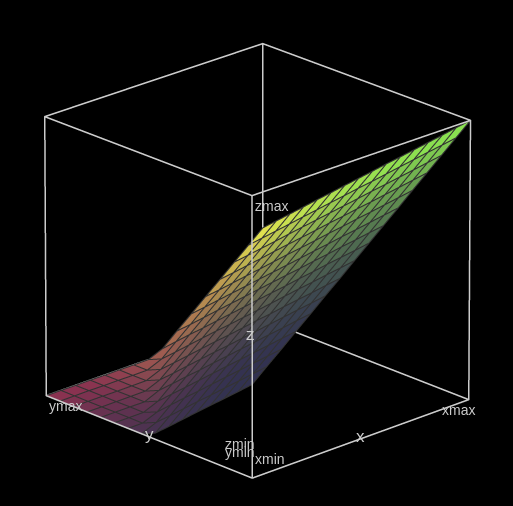
\includegraphics[width=5cm]{hinge}                                  
\end{frame}  

\begin{frame}{Margin}
  \[\frac{\bolddelta \mathcal{L}}{\bolddelta \theta_i} = \sum_i \boldy_i - \boldy_{\hat{c}}  \]
\end{frame}



\begin{frame}{Current State of the Art} 
  
\end{frame}

\end{document}

